\documentclass[11pt,a4paper]{scrartcl}
\usepackage[czech]{babel}
\usepackage[utf8]{inputenc}
\usepackage{graphicx}
\usepackage{float}

\begin{document}
	\title{Semestrální práce z předmětu KIV/DS}
	\subtitle{Globální stav v distribuovaném systému}
	\author{Zdeněk Valeš}
	\date{10.1. 2020}
	\maketitle
	\newpage
	
	\section{Zadání}
	Implementace ZeroMQ služby s integrovaným Chandy-Lmportovým algoritmem pro získání konzistentního snímku globálního stavu.
	
	Popis chodu aplikace:
	\begin{itemize}
		\item Implementujte bankovní službu s operacemi (lze využít implementaci z předchozí úlohy) credit a debit tak, že obě operace lze provést na základě zprávy doručené do vstupní ZeroMQ fronty následovně: pokud klient chce poslat částku do jiné banky, odečte částku a pošle zprávu CREDIT s částkou do jiné banky (fronty). Pokud chce klient inkasovat částku z jiné banky, pošle pouze zprávu DEBIT s částkou, přičemž druhá strana částku odečte a pošle ji ve zprávě CREDIT.

		\item Všechny uzly jsou identické, kromě IP adresy a jména uzlu, jejich počet je v rozmezí 2-5
		
		\item Každý uzel po startu začíná se zůstatkem na účtu 5.000.000.

		\item Uzly náhodně vyberou jednu z operací CREDIT či DEBIT s náhodnou částkou v intervalu <10.000, 50.000> a
		odešlou zprávu s operací na náhodně vybraný sousední uzel. Pokud uzel na svém účtu nemá dostatečnou
		částku, operaci odmítne.
		
		\item Uzly spolu komunikují pouze přes vstupní ZeroMQ fronty (podle vzoru PAIR, viz, které představují komunikační kanály. Zprávy
		přenášejte v JSON formátu
		
		\item Topologii si zvolte sami, ale je nutné ji uvést v průvodní dokumentaci
		
		\item Jako servisní službu implementujte Chandy-Lamportův distribuovaný algoritmus pro získání konzistentního snímku globálního stavu podle stejného principu jako bankovní API (zpráva “marker” ve vstupní frontě – viz popis algoritmu)

		\item Spuštění Chandy-Lamportova algoritmu zahajte posláním zprávy MARKER do libovolné fronty (z příkazové
		řádky na libovolném uzlu).

		\item Ošetřete i případ, že může být v jednom okamžiku spuštěno více snapshotů

		\item Stavem uzlu se rozumí zůstatek na účtu v okamžiku přijetí prvního markeru, stavem kanálu seznam zpráv s
		bankovními operacemi přijatými po prvním markeru (viz popis algoritmu)

		\item Jakmile detekujete ukončení algoritmu, všechny uzly pošlou svoje uložené stavy do vyhrazené fronty, ze které
		je vyhrazený proces vybírá a zobrazuje (stačí na konzoli)

		\item K vytvoření infrastruktury použijte nástroje Vagrant a VirtualBox

		\item Aplikaci můžete implementovat v Jazyce Java nebo Python s využitím již existujícího software, který vám
		usnadní implementaci jednotlivých modulů a jejich vzájemnou komunikaci.
	\end{itemize}
	
	
	
	\section{Popis implementace}
	K implementaci jsem si vybral jazyk Python (verze 3). Banky a služba pro sběr globálního stavu spolu navzájem komunikují skrze ZroMQ fronty. Systém obsahuje 4 bankovní servery a jednu službu pro sběr stavu.
	
	\subsection{Topologie systému}
	TODO
	Topologie systému, společně s IP adresou virtuálního stroje a portem, na kterém je přístupné REST API je znázorněna na obrázku \ref{fig:topology}. Každý virtuální stroj je založen na image \verb|ubuntu/trusty32| -- můj počítač nepodporuje virtualizaci 64 bitových systémů.
	
	Dokumentaci API jednotlivých serverů je přiložena v souborech \verb|sequencer-api.yml|, \verb|shuffler-api.yml| a \verb|bank-api.yml|.
	
	\begin{figure}[H]
		\centering
		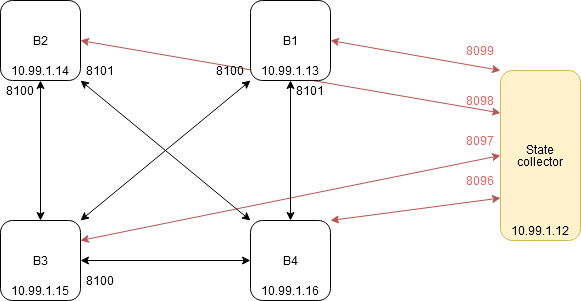
\includegraphics[width=15cm]{img/topologie.png}
		\caption{Topologie systému}
		\label{fig:topology.pdf_tex}
	\end{figure}

	\subsection{Konfigurace}
	TODO
	
	\subsection{Obecná struktura projektu}
	Zdrojové kódy projektu se nachází ve složce \verb|src|. Každý server je umístěn ve vlastní složce (\verb|client|, \verb|bank-1|, ...). V adresáři \verb|src| je také umístěn \verb|Vagrantfile| obsahující konfiguraci nasazení virtuálních strojů. 
	
	Server je tvořen python skriptem, konfiguračním souborem pro \verb|upstart| a skriptem \verb|bootstrap.sh|, který server inicializuje a spouští. Každý server je na virtuálním stroji veden jako služba. Tím je možné daný server pohodlně vypínat/zapínat. 	Každý ze serverů loguje svou činnost do souboru \verb|log.txt|, skrze který je možné za běhu kontrolovat stav systému. 
	
	\begin{figure}[H]
		\centering
%		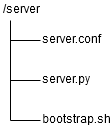
\includegraphics[width=2.5cm]{server-structure.png}
		\caption{Obecná struktura složky serveru}
		\label{fig:serv-struct.pdf_tex}
	\end{figure}
	
	\subsection{Bank N}
	Bankovní server přijímá pokyny k transakcím od shuffleru a ukládá je do interní haldy. Na vrchu této haldy je pokyn s nejmenším časovým razítkem (ta generuje sekvencer). Při spuštění bankovního serveru je nastaven interní čítač očekávaných id na hodnotu, která musí odpovídat prvnímu id generovanému sekvencerem. Pokud je na vrcholu haldy pokyn s $id = expected\_id$, je vyjmut a proveden. 	Po každé provedené transakci je do souboru \verb|balance.txt| zapsán současný zůstatek na účtě. 
	
	Vzhledem k nutnosti 'synchronizace' prvního id generovaného sekvencerem a počátečního \verb|expected_id| bankovního serveru je v případě restartu sekvenceru nutné restartovat také všechny bankovní servery (a naopak).
	
	Každý bankovní server má vlastní databázi běžící na daném virtuálním stroji.
	
	\subsubsection{Chandy-Lamport}
	TODO
	
	\subsection{Služba pro sběr stavů systému}
	TODO
	
	\section{Spuštění}
	TODO
	Systém je možné spustit příkazem \verb|vagrant up| v adresáři \verb|src|. Stav klienta je možné kontrolovat skrze ssh na vrituální stroj příkazem \verb|status client|. V případě, že klient doběhl, jeho status bude \verb|stop/waiting|.
	
	Po doběhnutí klienta lze zkontrolovat zůstatky bankovních serverů. Zůstatek je na každém serveru uložen v souboru \verb|/home/vagrant/bank/balance.txt|.
	
	\section{Závěr}
	TODO
	Práci se mi podařilo úspěšně implementovat. Míchání požadavků shufflerem by bylo lepší realizovat skrze náhodné zpoždění, systém by tak více odrážel reálný stav. Zapisovat aktuální zůstatek na účte do souboru po každé provedené transakci je není obecně dobrá praktika, ale zde to usnadňuje testování a kontrolu výsledků.
	
\end{document}
